\documentclass[12pt]{article}
\usepackage{enumitem}
\usepackage{setspace}
\usepackage{graphicx}
\usepackage{subcaption}
\usepackage{booktabs}
\usepackage{amsmath, amsthm}
\usepackage{amssymb}
\RequirePackage[colorlinks]{hyperref}
\usepackage[lined,boxed,linesnumbered,commentsnumbered]{algorithm2e}
\usepackage{xcolor}
\usepackage{listings}
\usepackage{subfloat}

\lstset{basicstyle=\ttfamily,
  showstringspaces=false,
  commentstyle=\color{red},
  keywordstyle=\color{blue}
}

% Margins
\topmargin=-0.45in
\evensidemargin=0in
\oddsidemargin=0in
\textwidth=6.5in
\textheight=9.0in
\headsep=0.25in

\linespread{1.1}

% Commands
\newenvironment{solution}
  {\begin{proof}[Solution]}
  {\end{proof}}

\newcommand{\snehaedit}[1]{\textcolor{green}{\emph{[Sneha: #1]}}}
\newcommand{\hsedit}[1]{\textcolor{magenta}{\emph{[Hang: #1]}}}
\newcommand{\meeraedit}[1]{\textcolor{red}{\emph{[Meera: #1]}}}
\newcommand{\prpedit}[1]{\textcolor{blue}{\emph{[Prp: #1]}}}


\title{CSE6250: Homework 2 Answer}
\author{Name: Yichao Zhang\\ GT User ID: yzhang3414}
\date{Deadline: Feb 3, 2019, 11:55 PM AoE}

\begin{document}

\maketitle

\section{Logistic Regression [25 points]}
\subsection{Batch Gradient Descent}


The negative log-likelihood can be calculated according to
\begin{equation}
NLL\left (D, \mathbf{w} \right ) = -\sum_{i=1}^{N} \left [ \left ( 1 - y_i \right ) \log(1-\sigma(\mathbf{w}^T\mathbf{x}_i)) + y_i\log \sigma(\mathbf{w}^T\mathbf{x}_i)  \right ]
\label{eq:NLL}
\end{equation}
where $\sigma(t) = \frac{1}{1 + e^{-t}}$ is the sigmoid function.\\

\textbf{a. Derive the gradient of the negative log-likelihood in terms of $\mathbf{w}$ for this setting. [5 points] }

$\because $
\begin{equation}
\frac{\partial}{\partial t}\sigma(t) 
= \frac{\partial}{\partial t}\frac{1}{1 + e^{-t}} 
= \frac{-1}{(1 + e^{-t})^2} \frac{\partial}{\partial t} e^{-t}
= \frac{e^{-t}}{(1 + e^{-t})^2}
= \sigma ( 1- \sigma)
\end{equation}

$\therefore$
\begin{equation}
\nabla_\mathbf{w}\sigma(\mathbf{w}^T\mathbf{x}_i) 
= \sigma ( 1- \sigma)\nabla_\mathbf{w} (\mathbf{w}^T\mathbf{x}_i)
= \sigma ( 1- \sigma)\mathbf{x}_i
\end{equation}

$\therefore$
\begin{equation}
\begin{aligned}
\nabla_\mathbf{w}NLL\left (D, \mathbf{w} \right ) 
& = -\sum_{i=1}^{N} \left [ 
\left ( 1 - y_i \right ) 
\nabla_\mathbf{w} \log(1-\sigma(\mathbf{w}^T\mathbf{x}_i)) 
+ y_i 
\nabla_\mathbf{w}\log \sigma(\mathbf{w}^T\mathbf{x}_i)  \right ] \\
& = -\sum_{i=1}^{N} \left [ 
-\left ( 1 - y_i \right ) \frac{1}{1-\sigma}
+ y_i \frac{1}{\sigma} 
\right ] \nabla_\mathbf{w} \sigma(\mathbf{w}^T\mathbf{x}_i) \\
& = -\sum_{i=1}^{N} \left [ 
-\left ( 1 - y_i \right ) \frac{1}{1-\sigma}
+ y_i \frac{1}{\sigma} 
\right ]
\sigma (1-\sigma)\mathbf{x}_i\\
& = -\sum_{i=1}^{N} \left [ 
-\left ( 1 - y_i \right ) \sigma
+ y_i (1-\sigma)
\right ]\mathbf{x}_i\\
& = -\sum_{i=1}^{N} \left [ 
y_i - \sigma(\mathbf{w}^T\mathbf{x}_i)
\right ]\mathbf{x}_i\\
\end{aligned} 
\label{eq:GradNLL}
\end{equation}


\subsection{Stochastic Gradient Descent}
If $N$ and $d$ are very large, it may be prohibitively expensive to consider every patient in $D$ before applying an update to $\mathbf{w}$. One alternative is to consider stochastic gradient descent, in which an update is applied after only considering a single patient. \\

\textbf{a. Show the log likelihood, $l$, of a single $(\mathbf{x}_t, y_t)$ pair. [5 points]}

From eq(\ref{eq:NLL}), by simply removing the summation, we get the log likelihood for a single patient :
\begin{equation}
\begin{aligned}
nll\left (D_t, \mathbf{w} \right ) = - \left [ \left ( 1 - y_t \right ) \log(1-\sigma(\mathbf{w}^T\mathbf{x}_t)) + y_t\log \sigma(\mathbf{w}^T\mathbf{x}_t)  \right ]
\end{aligned}
\label{eq:nll}
\end{equation}\\

\textbf{b. Show how to update the coefficient vector $\mathbf{w}_t$ when you get a patient feature vector $\mathbf{x}_t$ and physician feedback label $y_t$ at time $t$ using $\mathbf{w}_{t-1}$ (assume learning rate $\mathbf{\eta}$ is given). [5 points]}

From eq(\ref{eq:GradNLL}), by simply removing the summation, we get the gradient of a single patient:
\begin{equation}
\begin{aligned}
\nabla_\mathbf{w}nll\left (D_t, \mathbf{w} \right ) 
& = - \left [ 
y_t - \sigma(\mathbf{w}^T\mathbf{x}_t)
\right ]\mathbf{x}_t\\
\end{aligned} 
\end{equation}

$\therefore$ to minimize the negative log likelihood of a single patient, we update the $\mathbf{w}$ by
\begin{equation}
\begin{aligned}
\mathbf{w}_{t}
& =  \mathbf{w}_{t-1} - \eta \nabla_\mathbf{w}nll\left (D_t, \mathbf{w} \right )
\bigg|_{\mathbf{w} = \mathbf{w}_{t-1} } \\
& = \mathbf{w}_{t-1}
+ \eta \left [ 
y_t - \sigma(\mathbf{w}_{t-1}^T\mathbf{x}_t)
\right ]\mathbf{x}_t\\
\end{aligned} 
\end{equation}


\textbf{c. What is the time complexity of the update rule from $\mathbf{b}$ if $\mathbf{x}_t$ is very sparse? [2 points]}
\begin{itemize}

\item Update for a single patient in 1 iteration:

We need to update each component of $\mathbf{w}_t$ where the respective component of $\mathbf{x}_t$ is non-zero. Suppose  $\mathbf{x}_t$ has $m$ non-zero components in average, then the time complexity is $O(m)$.

If $\mathbf{x}_t$ is very sparse, then $m \rightarrow 1$, it becomes $O(1)$.

\item Update for N patient in 1 iteration:

The time complexity is $O(m N)$.

Similarly, if $\mathbf{x}_t$ is very sparse, the time complexity becomes $O(N)$

\item Update for $I$ iterations:

The time complexity is $O(m N I )$.

Similarly, if $\mathbf{x}_t$ is very sparse, the time complexity becomes $O(N I)$\\
\end{itemize}



\textbf{d. Briefly explain the consequence of using a very large $\mathbf{\eta}$ and very small $\mathbf{\eta}$. [3 points]}


A very large learning rate $\mathbf{\eta}$ means we update $\mathbf{w}$ by very large steps, so SGD may not converge to the minimum. And SGD may finish searching in a few iterations, or never stop.

A very small learning rate $\mathbf{\eta}$ means we update $\mathbf{w}$ by very small steps, so it may take much more iterations for SGD to converge to the minimum.\\


\textbf{e. Show how to update $\mathbf{w}_t$ under the penalty of L2 norm regularization. In other words, update $\mathbf{w}_t$ according to $l - \mu \|\mathbf{w}\|_2^2 $, where $\mathbf{\mu}$ is a constant. What's the time complexity? [5 points]}

When we add a penalty term: $- \mu \|\mathbf{w}\|_2^2 $ to the log likelihood for single patient, the negative log likelihood for single patient becomes: $nll\left (D_t, \mathbf{w} \right ) + \mu \|\mathbf{w}\|_2^2 $.

$\because$
\begin{equation}
\begin{aligned}
\nabla_\mathbf{w}\|\mathbf{w}\|_2^2 = \nabla_\mathbf{w}(\mathbf{w}^T \mathbf{w}) = 2 \mathbf{w}
\end{aligned} 
\end{equation}

$\therefore$ we update $\mathbf{w}$ by:
\begin{equation}
\begin{aligned}
\mathbf{w}_{t}
& =  \mathbf{w}_{t-1} - \eta \nabla_\mathbf{w}\bigg[ nll\left (D_t, \mathbf{w} \right ) + \mu \|\mathbf{w}\|_2^2 \bigg]
\bigg|_{\mathbf{w} = \mathbf{w}_{t-1} } \\
& =  \mathbf{w}_{t-1} - \eta \nabla_\mathbf{w} nll\left (D_t, \mathbf{w} \right ) - \eta  \mu \nabla_\mathbf{w}\|\mathbf{w}\|_2^2 
\bigg|_{\mathbf{w} = \mathbf{w}_{t-1} } \\
& = \mathbf{w}_{t-1}
+ \eta \left [ 
y_t - \sigma(\mathbf{w}_{t-1}^T\mathbf{x}_t)
\right ]\mathbf{x}_t
- 2 \eta \mu \mathbf{w}_{t-1}\\
\end{aligned} 
\end{equation}

Time complexity:
\begin{itemize}
\item For a single patient in 1 iteration: we need to update each component of $\mathbf{w}_t$, no matter $\mathbf{x}_t$ is sparse or not. Here $\mathbf{w} \in \mathbf{R}^d$ , so the time complexity is $O(d)$.

\item For N patient in 1 iteration: the time complexity is $O(d N)$.

\item For $I$ iterations: the time complexity is $O(d N I)$.\\

\end{itemize}


%\textbf{f.} When you use L2 norm, you will find each time you get a new $(\mathbf{x}_t, y_t)$ you need to update every element of vector $\mathbf{w}_t$ even if $\mathbf{x}_t$ has very few non-zero elements. Write the pseudo-code on how to update $\mathbf{w}_t$ lazily. [Extra 5 points] \textbf{(no partial credit!)} \\

%\textbf{HINT}: Update $j$-th element of $\mathbf{w}_{t}$, $\mathbf{w}_{tj}$, only when $j$-th element of $\mathbf{x}_{t}$, $\mathbf{x}_{tj}$, is non-zero. You can refer to Sec.10 and 11 and the appendix of this \href{http://lingpipe.files.wordpress.com/2008/04/lazysgdregression.pdf}{paper}. 

\section{Programming [75 points]}

%\begin{lstlisting}[frame=single,language=python]
%source /scripts/switch-to-py3
%\end{lstlisting}

%Keep in mind you will need to run the corresponding \textbf{switch-to-py3} script if you want to switch back to Python 3. \\

%\textbf{Please ensure you are always using Python 3.6.5 for the remainder of the assignment or you may encounter problems!}


\subsection{Descriptive Statistics [15 points]}


\begin{table}[th]
\centering
\begin{tabular}{@{}l|l|l}
\toprule
Metric & Deceased patients & Alive patients  \\ \hline
Event Count & & \\ 
1. Average Event Count & 1027.739 & 683.155 \\
2. Max Event Count  & 16829 & 12627\\
3. Min Event Count  & 2 & 1\\ \hline

Encounter Count & & \\ 
1. Average Encounter Count  & 24.839 & 18.695\\
2. Max Encounter Count  & 375 & 391 \\
3. Min Encounter Count  & 1 & 1 \\ \hline

Record Length & &  \\ 
1. Average Record Length & 157.042 & 194.703\\
2. Median Record Length & 25 & 16 \\
3. Max Record Length& 5364 & 3103 \\
4. Min Record Length& 0 & 0 \\ \hline

Common Diagnosis & DIAG320128 & DIAG320128 \\ 
				& DIAG319835 & DIAG319835 \\ 
				& DIAG313217 & DIAG317576 \\
				& DIAG197320 & DIAG42872402 \\
				& DIAG132797 & DIAG313217 \\ \hline

Common Laboratory Test & LAB3009542 & LAB3009542 \\ 
					& LAB3023103 & LAB3000963 \\ 
					& LAB3000963 & LAB3023103 \\ 
					& LAB3018572 & LAB3018572 \\
					& LAB3016723 & LAB3007461 \\ \hline

Common Medication & DRUG19095164 & DRUG19095164 \\ 
				& DRUG43012825 & DRUG43012825 \\ 
				& DRUG19049105 & DRUG19049105 \\ 
				& DRUG956874 & DRUG19122121 \\
				& DRUG19122121 & DRUG956874 \\ \hline
\bottomrule
\end{tabular}
\caption{Descriptive statistics for alive and dead patients\label{tbl:stat}}
\end{table} 


\subsection{Transform data [20 points]}
\subsection{SGD Logistic Regression [20 points]}

Train and test a classifier by running 
\begin{enumerate}
\item cat ../pig/training/part-r-00000 \textbar{} python train.py -f 3618
\item cat ../pig/testing/part-r-00000 \textbar{} python test.py 
\end{enumerate}

\textbf{b. Show the ROC curve generated by test.py in this writing report for different learning rates $\eta$ and regularization parameters $\mu$ combination and briefly explain the result. [5 points]}
\begin{figure}[ht!]
    \centering
    \begin{subfigure}{.4\linewidth}
        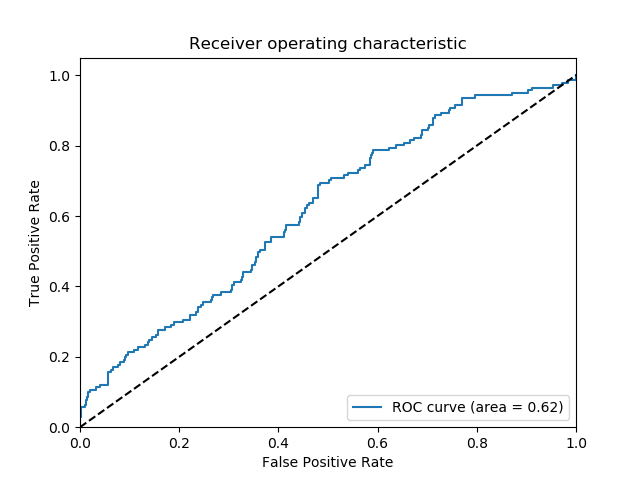
\includegraphics[scale=0.5]{roc_0_01_0_0.png}
        \caption{$\eta = 0.01, \mu = 0, ROC = 0.62$}
    \end{subfigure}
    \hskip2em
    \begin{subfigure}{.4\linewidth}
        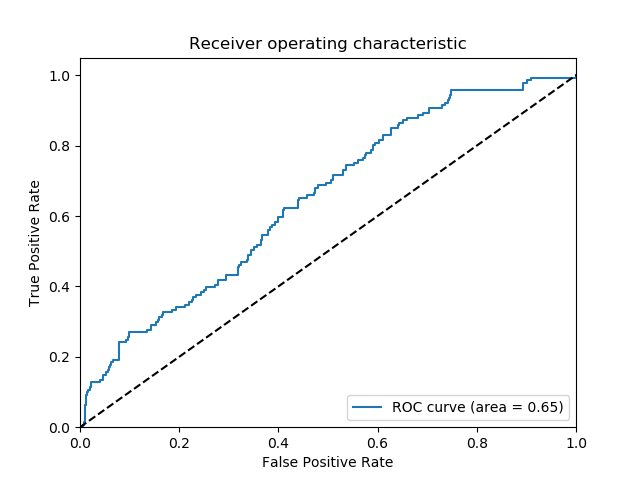
\includegraphics[scale=0.5]{roc_0_1_0_0.png}
        \caption{$\eta = 0.1, \mu = 0, ROC = 0.65$}
    \end{subfigure}
    \begin{subfigure}{.4\linewidth}
        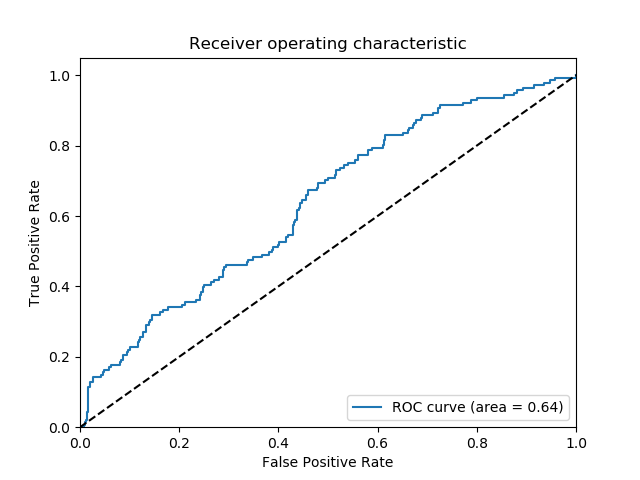
\includegraphics[scale=0.5]{roc_0_2_0_0.png}
        \caption{$\eta = 0.2, \mu = 0, ROC = 0.64$}
    \end{subfigure}
    \caption{Tune $\eta$, with fixed $\mu = 0$ }
\end{figure}

Firstly, I fixed $\mu = 0$, and tune the learning rate $\eta$ from 0.01 to 0.2. I find that the highest ROC score (0.65) is on $\eta = 0.1$. If the learning rate is higher than 0.1, it may not converge to the minimum. And if it is much lower than 0.1, then it cannot finish searching minimum in short times.

\begin{figure}[ht!]
    \centering
    \begin{subfigure}{.4\linewidth}
        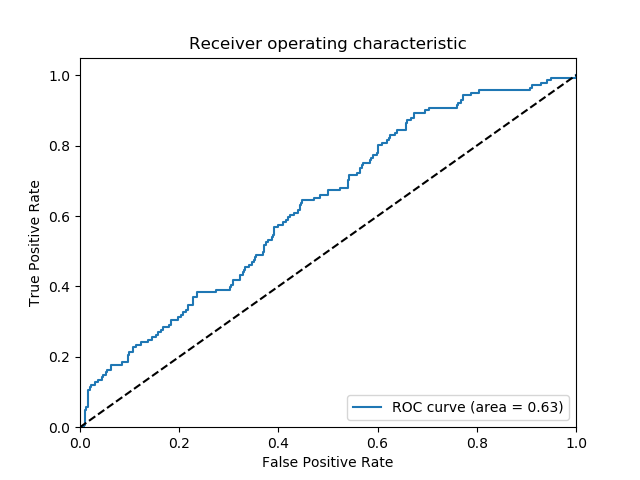
\includegraphics[scale=0.5]{roc_0_1_0_01.png}
        \caption{$\eta = 0.1, \mu = 0.01, ROC = 0.63$}
    \end{subfigure}
    \hskip2em
    \begin{subfigure}{.4\linewidth}
        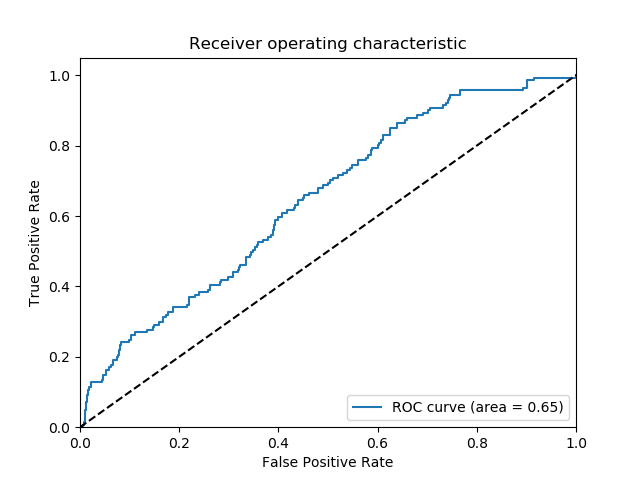
\includegraphics[scale=0.5]{roc_0_1_0_001.png}
        \caption{$\eta = 0.1, \mu = 0.001, ROC = 0.65$}
    \end{subfigure}
    \caption{Tune $\mu$, with fixed $\eta = 0.1$ }
\end{figure}

Secondly, I fixed $\eta = 0.01$, and tried some different L2 penalty constant $\mu$. When $\mu$ is a little large, like 0.1, the ROC performance decrease due to the trade-off between optimizing the parameters and simplifying the parameters.

When $\mu$ is very small, like 0.001, the performance is as good as $\mu = 0$. However, the penalty term makes the parameters smaller and simpler. Considering the Occam's Razor principle, this model is likely to have a better generalizability. 

\newpage
\subsection{Hadoop [15 points]}
\textbf{c. Compare the performance with that of previous problem and briefly analyze why the difference. [5 points]}


\begin{figure}[ht!]
    \centering
    \begin{subfigure}{.4\linewidth}
        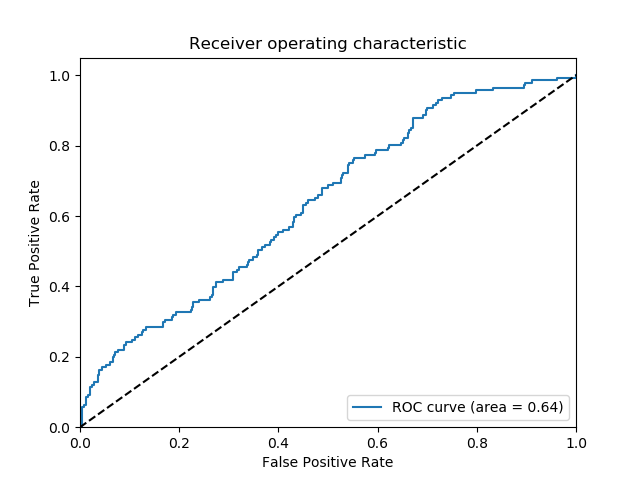
\includegraphics[scale=0.5]{roc_ensemble_0_1_0_001.png}
        \caption{$\eta = 0.1, \mu = 0.001, ROC = 0.64$}
    \end{subfigure}
    \hskip2em
    \begin{subfigure}{.4\linewidth}
        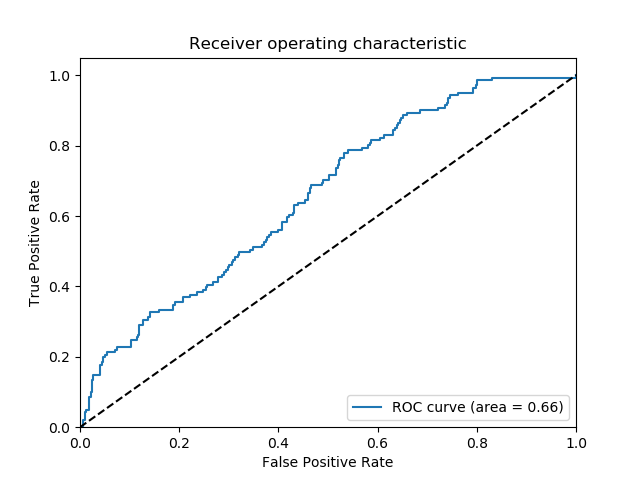
\includegraphics[scale=0.5]{roc_ensemble_0_4_0_001.png}
        \caption{$\eta = 0.4, \mu = 0.001, ROC = 0.66$}
    \end{subfigure}
    \caption{ROC performance of ensemble models, model number $n = 5$, sample ratio $r = 0.4$ }
\end{figure}

By using the best parameter in the single model: $\eta = 0.1, \mu = 0.001$, the ROC score of ensemble model is 0.64, lower than the single model, which has 0.65.

However, when I increased the learning rate $\eta$ to $0.4$, the ROC of ensemble model raised to 0.66,  better than single model. That means the single model with small value of $\eta=0.1$ may overfits the training data. In addition, the larger value of learning rate increase the speed of ensemble model.

\end{document}
\end{document}